\definecolor{acmBlue}{HTML}{1F77B4}
\definecolor{acmTeal}{HTML}{009E73}
\definecolor{acmSand}{HTML}{D55E00}
\definecolor{acmGray}{HTML}{8A8F99}
\definecolor{acmGrid}{HTML}{D9DDE2}
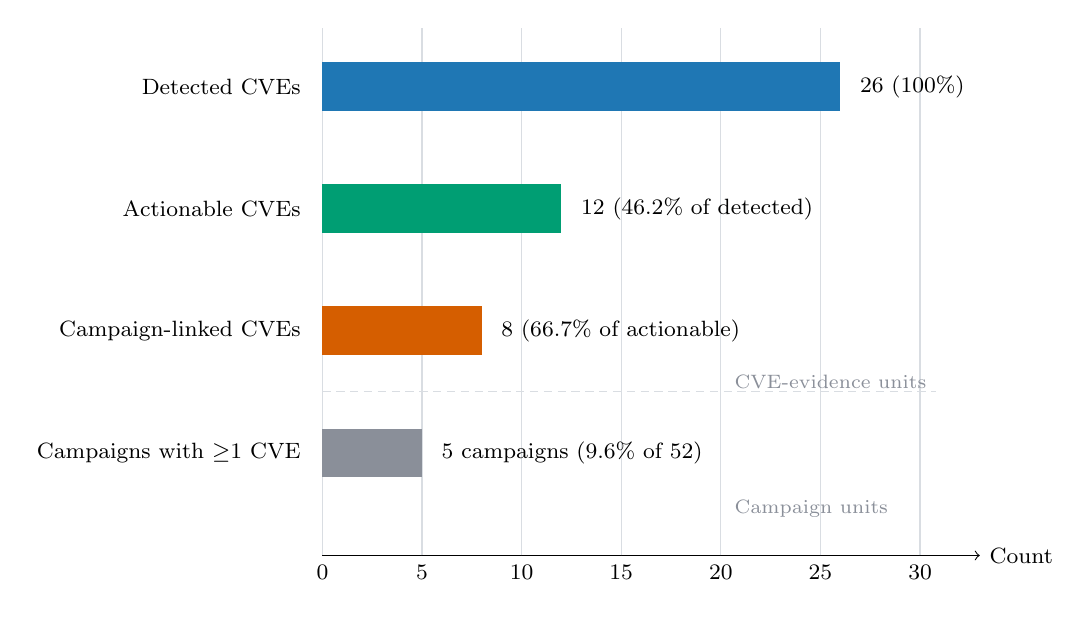
\begin{tikzpicture}[x=0.253cm,y=0.62cm,font=\footnotesize]
  \draw[->] (0,0) -- (33.0,0) node[right] {Count};
  \foreach \x in {0,5,10,15,20,25,30} {
    \draw[acmGrid] (\x,0) -- (\x,10.8);
    \node[below] at (\x,0) {\x};
  }
  \node[anchor=east] at (-0.6,9.6) {Detected CVEs};
  \node[anchor=east] at (-0.6,7.1) {Actionable CVEs};
  \node[anchor=east] at (-0.6,4.6) {Campaign-linked CVEs};
  \node[anchor=east] at (-0.6,2.1) {Campaigns with $\geq$1 CVE};
  \fill[acmBlue] (0,9.1) rectangle (26,10.1);
  \fill[acmTeal] (0,6.6) rectangle (12,7.6);
  \fill[acmSand] (0,4.1) rectangle (8,5.1);
  \fill[acmGray] (0,1.6) rectangle (5,2.6);
  \draw[densely dashed,acmGrid] (0,3.35) -- (30.8,3.35);
  \node[anchor=west,font=\scriptsize,text=acmGray] at (20.2,3.55) {CVE-evidence units};
  \node[anchor=west,font=\scriptsize,text=acmGray] at (20.2,0.95) {Campaign units};
  \node[anchor=west] at (26.5,9.6) {26 (100\%)};
  \node[anchor=west] at (12.5,7.1) {12 (46.2\% of detected)};
  \node[anchor=west] at (8.5,4.6) {8 (66.7\% of actionable)};
  \node[anchor=west] at (5.5,2.1) {5 campaigns (9.6\% of 52)};
\end{tikzpicture}
